\section{Task 2}

In this task, I placed the phone on the table without any touch or movement. 

When the phone is placed flat on a table, the accelerometer should read the gravitational acceleration on the Z-axis, while the readings on the X and Y axes should be zero.
The readings of the gyroscope should be zero in all three directions, while the magnetometer readings should reflect the magnetic field strength of the phone's current position.

Just note myself: 3pm 5.24 from library

Since the last moment I touched the screen to stop stream, so in calculation I should remove a little bit tail data.

\subsection{True state}

\begin{figure}[H]
 \centering
 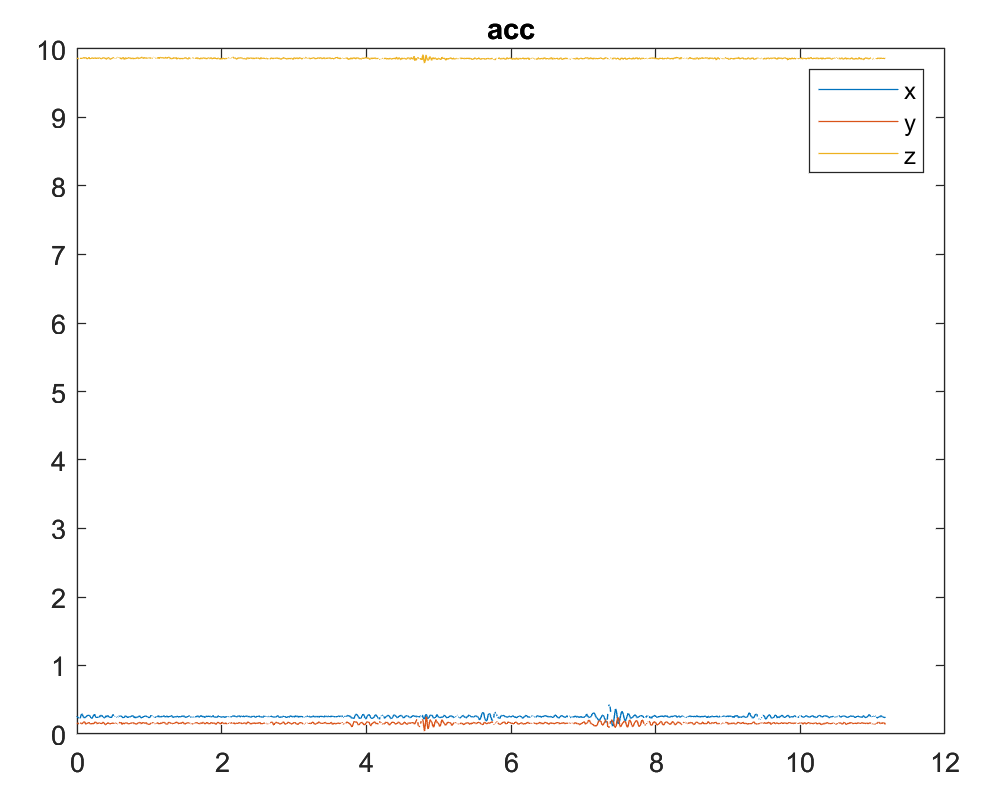
\includegraphics[width=0.7\textwidth]{images/acc.png}
 \caption{Accelerometers}
 \label{acc}
\end{figure}

\begin{figure}[H]
 \centering
 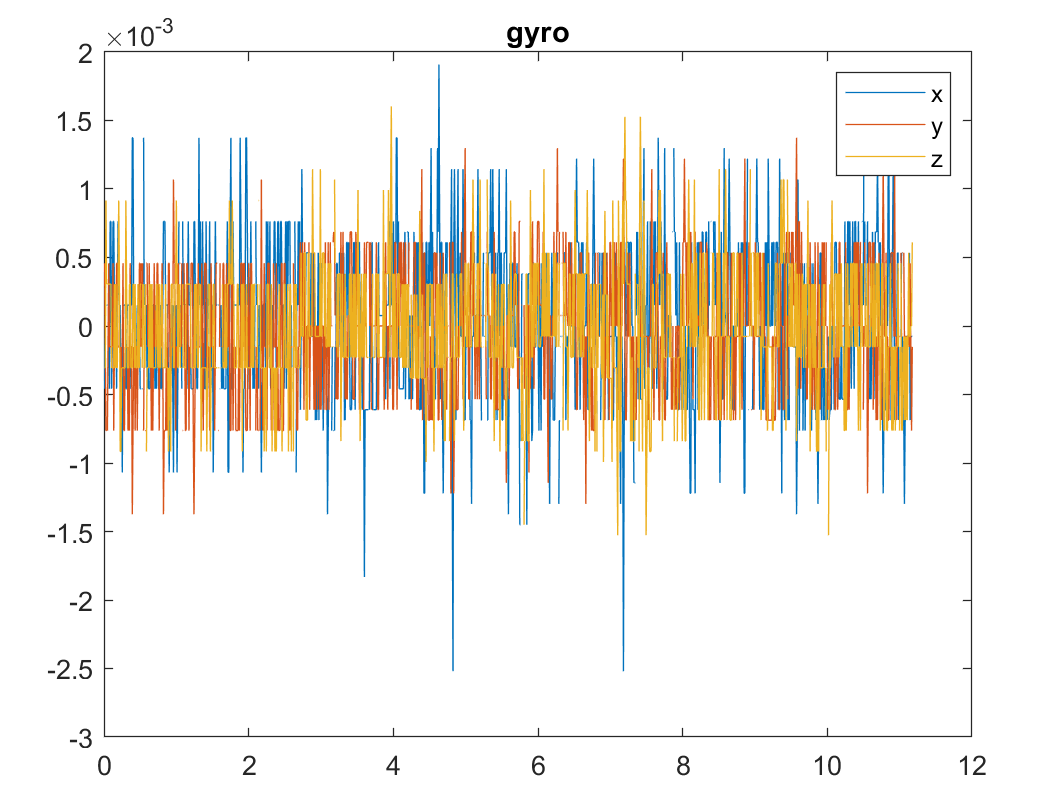
\includegraphics[width=0.7\textwidth]{images/gyroscope.png}
 \caption{Gyroscope}
 \label{gyro}
\end{figure}

\begin{figure}[H]
 \centering
 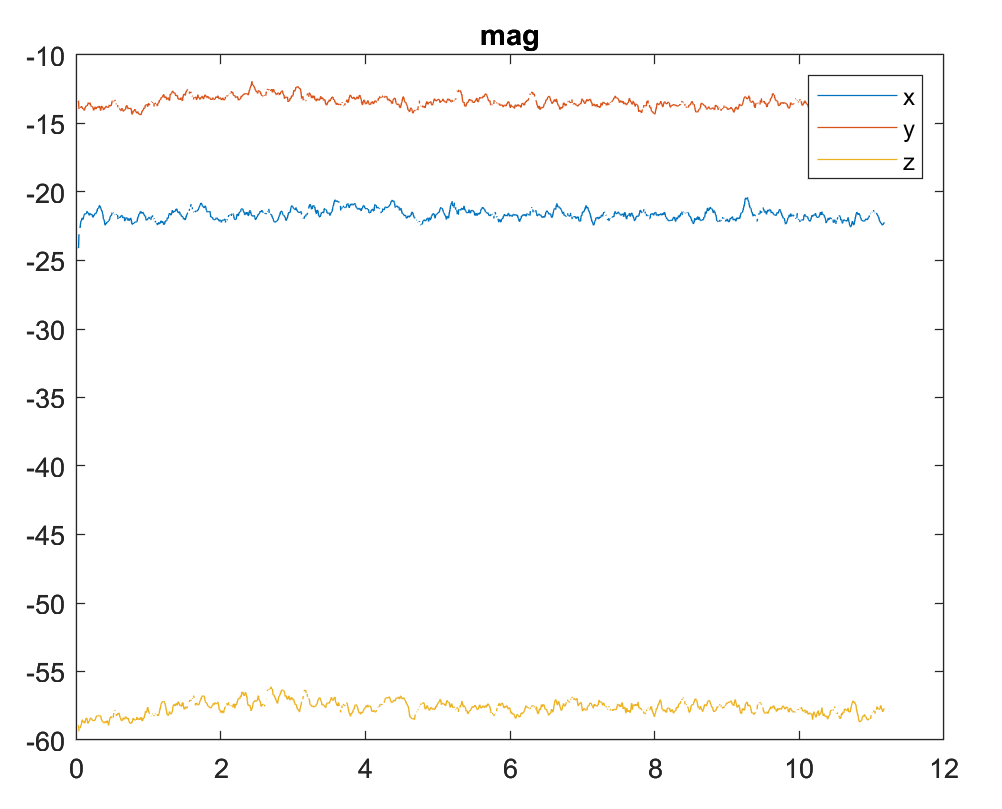
\includegraphics[width=0.7\textwidth]{images/magnetometers.png}
 \caption{Magnetometers}
 \label{mag}
\end{figure}

By observing the plots of the sensors, it can be noted that when the phone is placed flat on a table, the readings from all three sensors exhibit a stable trend without significant disturbances.

\subsection{Mean and covariance and histograms}

\begin{figure}[H]
 \centering
 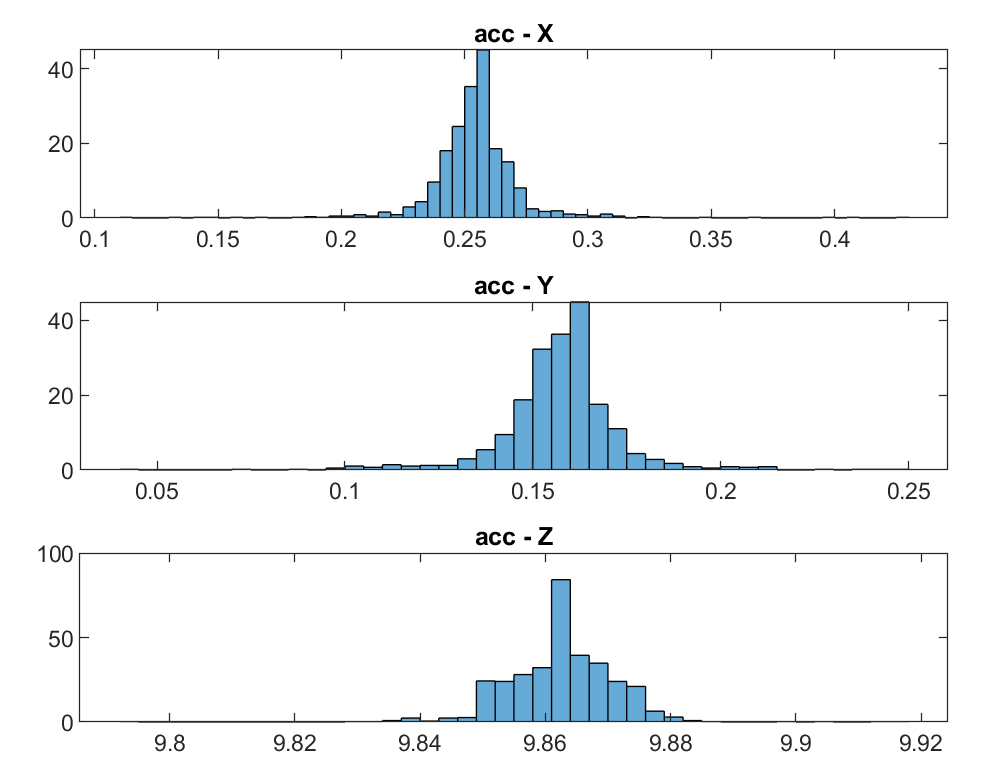
\includegraphics[width=0.7\textwidth]{images/histogramacc.png}
 \caption{Histograms for accelerometers}
 \label{hisacc}
\end{figure}

The mean of acc -X is 0.254171 , the covariance of acc -X is 0.019724  

The mean of acc -Y is 0.157052 , the covariance of acc -Y is 0.016096 

The mean of acc -Z is 9.862452 , the covariance of acc -Z is 0.008445 

\begin{figure}[H]
 \centering
 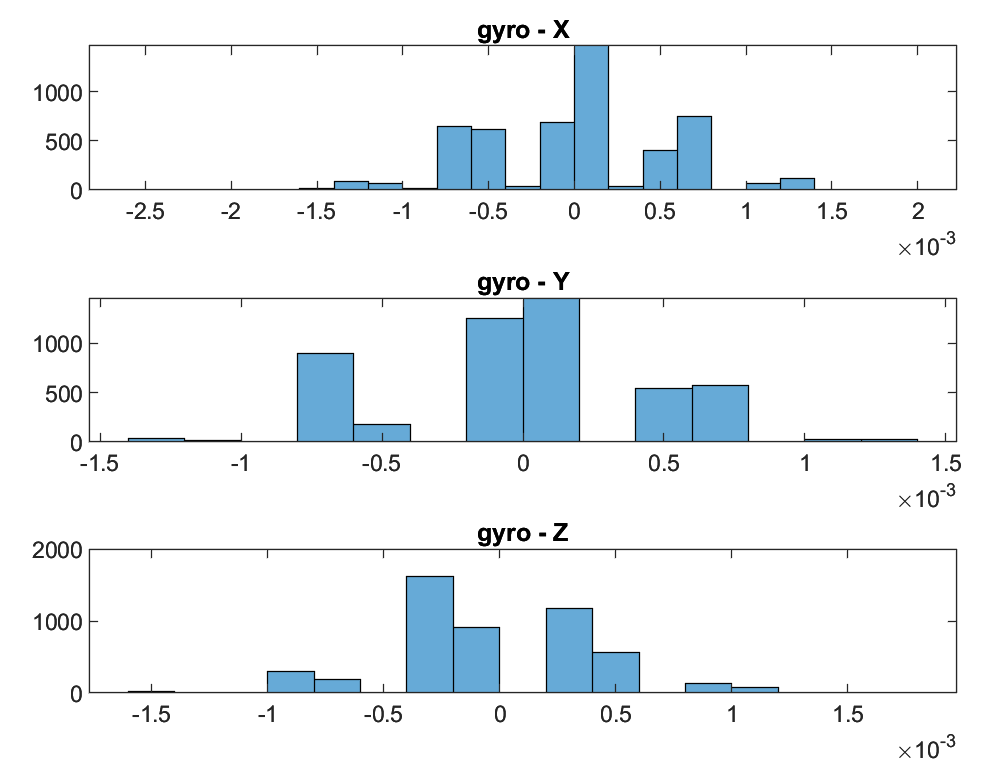
\includegraphics[width=0.7\textwidth]{images/histogramgyroscope.png}
 \caption{Histograms for gyroscope}
 \label{hisgyro}
\end{figure}


The mean of gyro -X is 0.000014 
, the covariance of gyro -X is 0.000554  

The mean of gyro -Y is -0.000031 
, the covariance of gyro -Y is 0.000449 

The mean of gyro -Z is -0.000025 
, the covariance of gyro -Z is 0.000453 

\begin{figure}[H]
 \centering
 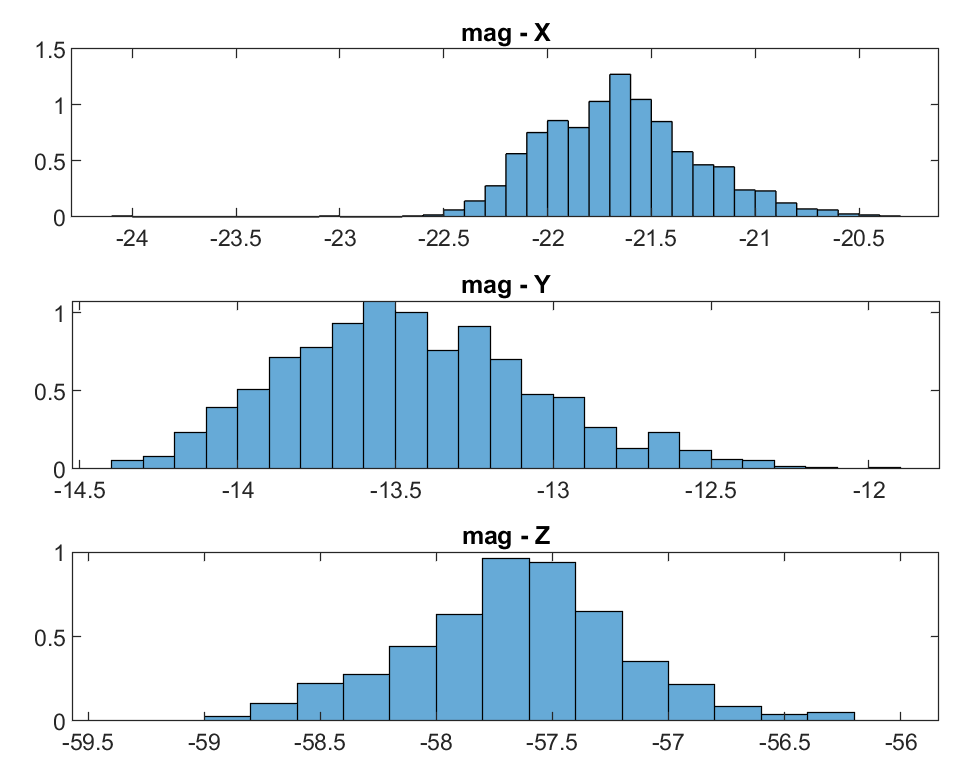
\includegraphics[width=0.7\textwidth]{images/hismagnetometer.png}
 \caption{Histograms for magnetometers}
 \label{hismag}
\end{figure}

The mean of mag -X is -21.648532 
, the covariance of mag -X is 0.377973  

The mean of mag -Y is -13.445163 
, the covariance of mag -Y is 0.401212 

The mean of mag -Z is -57.647071 
, the covariance of mag -Z is 0.477309 




The histogram of the accelerometer (acc) exhibits a shape close to a Gaussian distribution, with a small offset around the mean. This offset may be attributed to initial calibration errors present during sensor measurements. Considering the protrusion of the rear camera on my phone, the mean offset of the accelerometer is likely caused by the components of gravitational acceleration along the corresponding coordinate axes. Since the phone is unlikely to be placed on a table for measurements in future use, this error can be avoided. Therefore, it is reasonable to treat the noise in the accelerometer as Gaussian noise.

The histogram of the gyroscope (gyro) does not perfectly match a Gaussian distribution. This discrepancy could be due to the gyroscope's measurement errors being extremely small. Even if there are some offsets, the histogram shape may not be as pronounced as a Gaussian distribution due to the minimal presence of noise.
The noise in the gyroscope is extremely small. During the subsequent tuning process, it can be considered completely reliable, and its measurement model's noise can be set to zero.


The histogram of the magnetometer (mag) exhibits a shape similar to a Gaussian distribution but with an overall offset. This offset may be caused by environmental noise in the magnetic field or biases in the magnetometer.
The magnetometer should be calibrated based on the current environment before each use, depending on the specific requirements of the subsequent content.



